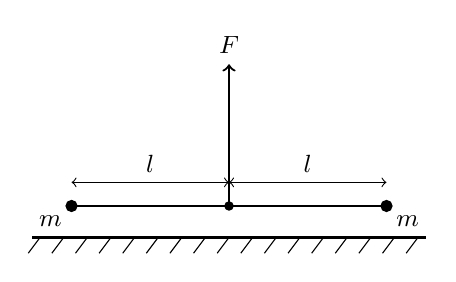
\begin{tikzpicture}[font=\small]
  % 两球用绳连接，绳中点受力F
  \filldraw (0,0) circle (2pt) node[below left] {$m$};
  \filldraw (4,0) circle (2pt) node[below right] {$m$};
  \draw[thick] (0,0) -- (4,0);
  % 绳中点
  \filldraw (2,0) circle (1.5pt);
  \draw[->, thick] (2,0) -- (2,1.8) node[above] {$F$};
  % 绳长标注
  \draw[<->] (0,0.3) -- (2,0.3) node[midway, above] {$l$};
  \draw[<->] (2,0.3) -- (4,0.3) node[midway, above] {$l$};
  % 光滑水平面
  \draw[thick] (-0.5,-0.4) -- (4.5,-0.4);
  \foreach \x in {-0.4,-0.1,...,4.4}
    \draw (\x,-0.4) -- (\x-0.15,-0.6);
\end{tikzpicture}
